\section{Charged Pion Identification}

Charged pions are identified and separated from kaons, protons, and electrons by the amount of energy they lose in the TPC.  The dE/dx of a TPC track is obtained by sorting the hits according to energy loss, tossing out the top 30\%, and averaging the rest.  Track dE/dx values for a given particle species at a fixed momentum are Gaussian, so we can also express the dE/dx value for each track in terms of a deviation from the mean dE/dx for some identified particle at that track's momentum.  In particular, track energy loss values at STAR are commonly given in terms of ``$n\sigma(\pi)$'', the deviation from the mean of the pion peak divided by the width of the pion peak.  Protons and kaons fall to the left of the pion peak (lower energy loss) and electrons fall to the right (higher energy loss).

It turns out there is some significant time dependence in the $n\sigma(\pi)$ distributions.  Rather than assume a fixed mean of 0.0 for the pion Gaussian,  we performed a triple Gaussian fit on the $n\sigma(\pi)$ distribution for each fill and extracted time-dependent means to better calibrate the PID cut.  After this recalibration we can extract yields for the various species of charged particles by fitting the $n\sigma(\pi)$ distributions with a multi-Gaussian parametric function.  We start with 8 Gaussians -- one each for $\pi^{+}$, $\pi^{-}$, $K^{+}$, $K^{-}$, $p$, $\bar{p}$, $e^{+}$, and $e^{-}$.  We can reduce the number of free parameters by applying the following constraints:

\begin{itemize}
    \item all widths must be equal (dE/dx resolution isn't particle-dependent)
    \item particle/antiparticle pairs should have the same mean
    \item $\pi - K$, $\pi - p$, and $\pi - e$ separations are known from other analyses -- we can use them as input parameters
\end{itemize}

In the end we have 24 - 7 - 4 - 3 = 10 free parameters in the fit:  the Gaussian width, the mean of the $\pi$ peak, and the yields.  The particle separations change as a function of momentum, not $p_{T}$, so we slice each $p_{T}$ bin into momentum bins and fit each one individually.  Figure \ref{fig:typical-nsigmapi} shows a ``typical" fit result.  Note that the tracks have been shifted by 6*track.charge() in order to plot positive and negative charges on the same histogram.

\begin{figure}
  \begin{center}
    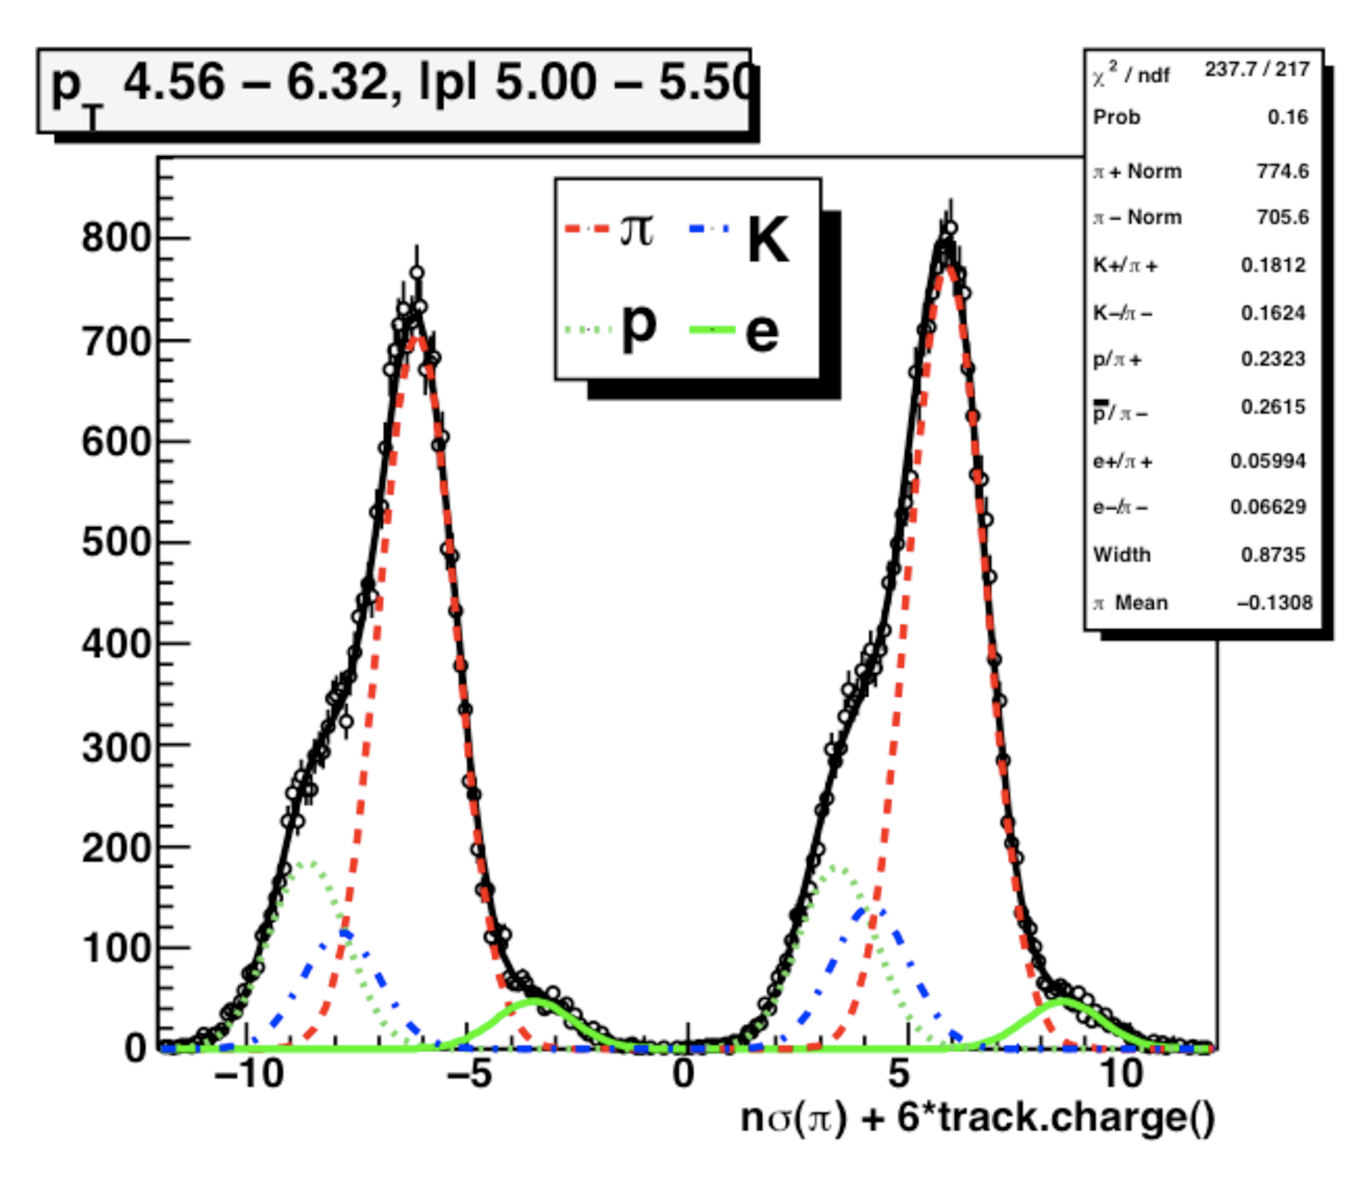
\includegraphics[width=0.7\textwidth]{figures/typical-nsigmapi}    
  \end{center}
  \caption{Example PID fit result}
  \label{fig:typical-nsigmapi}
\end{figure}

With this database of particle yields in hand we can calculate the set of PID cuts that minimize the statistical uncertainty on the background-subtracted $A_{LL}$ (Equation \ref{eqn:sigma-all}).  We wrote a simple minimization routine assuming $\sigma_{A_{LL}}^{2} = 1/N$ for the raw asymmetries and obtained the results in Table \ref{tbl:pid-selection-windows}.

\begin{table}
    \begin{center}
        \begin{tabular}{c|ccc}
        \hline
        $p_{T}$ bin & $\pi$ window & proton/kaon max & electron min\\
        \hline
        \hline
        [2.00 - 3.18] & (-1.10, 2.30) & -2.10 & 2.60\\
        \hline
        [3.18 - 4.56] & (-1.40, 2.10) & -2.10 & 2.40\\
        \hline
        [4.56 - 6.32] & (-1.40, 1.80) & -2.10 & 2.40\\
        \hline
        [6.32 - 8.80] & (-1.40, 1.80) & -2.10 & 2.40\\
        \hline
        [8.80 - 12.84] & (-1.30, 1.40) & -2.10 & 2.10\\
    \hline
    \end{tabular}
    \end{center}
    \caption{PID Selection Windows}
    \label{tbl:pid-selection-windows}
\end{table}
